\begin{frame}
\frametitle{Quantum information is fragile}

\begin{figure}
  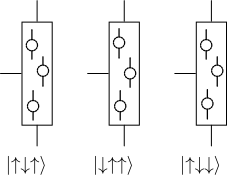
\includegraphics[scale=0.8]{transistors_microscopic.pdf}
  \caption*{Transistor with three electrons}
\end{figure}


First election scatters with a phonon:
$\ket{\mathcolor{red}{\uparrow} \uparrow \uparrow}\ket{0} \rightarrow \ket{\mathcolor{red}{\downarrow} \uparrow \uparrow}\ket{\mathcolor{red}{1}}$.

\pause
Superpostion of two transistors: $\ket{\uparrow \uparrow \uparrow} \ket{\downarrow \downarrow \downarrow} + \ket{\downarrow \downarrow \downarrow} \ket{\uparrow \uparrow \uparrow }$

first one subjected to scattering:
$$
\left( \ket{\mathcolor{red}{\uparrow} \uparrow \uparrow} \ket{\downarrow \downarrow \downarrow}
+ \ket{\downarrow \downarrow \downarrow} \ket{\uparrow \uparrow \uparrow} \right) \ket{0}
\longrightarrow
\ket{\mathcolor{red}{\downarrow} \uparrow \uparrow} \ket{\downarrow \downarrow \downarrow} \ket{\mathcolor{red}{1}}
+ \ket{\downarrow \downarrow \downarrow} \ket{\uparrow \uparrow \uparrow} \ket{0}
$$

\pause
Phonon states $\ket{0}$ and $\ket{1}$ orthogonal. Transistors now in \emph{classical} mixture of $\ket{\downarrow \uparrow \uparrow} \ket{\downarrow \downarrow \downarrow}$ and $\ket{\downarrow \downarrow \downarrow} \ket{\uparrow \uparrow \uparrow}$.
\pause

One single scattering even destroyed quantum coherence.
\end{frame}
